\documentclass[RNAAS]{aastex701}

\submitjournal{RNAAS}

\shorttitle{$\tau$ Ceti planets re-examined}
\shortauthors{Filatova et al.}

\graphicspath{{./}{figures/}}

\begin{document}

\title{$\tau$ Ceti's radial-velocity planets re-examined: cross-validated K-deficit, bimodal candidate~f, and a Bayes-factor reversal at higher nested-sampling resolution}

\author[0009-0007-3246-0182]{Vira Filatova}
\affiliation{DeepX, \url{https://deepxhub.com}}
\email{vira@deepxhub.com}

\author[0009-0001-5205-5519]{Taras Filatov}
\affiliation{DeepX, \url{https://deepxhub.com}}
\email{taras@deepxhub.com}

\begin{abstract}
\noindent
We re-analyse 23~years of multi-instrument radial-velocity (RV) data for $\tau$~Ceti (HARPS, HIRES, ESPRESSO, APF; 1\,275~nightly bins) within a joint Bayesian framework with an activity Gaussian process (GP), validated against the \texttt{RadVel} package \citep{Fulton2018}. Three of the four candidate planets reported by \citet{Feng2017} are confirmed by Bayesian evidence ($\Delta\log Z \gtrsim 4$); the fourth (candidate~f, $P\!\approx\!756$~d) shows a genuinely bimodal $K$ posterior. Our recovered semi-amplitudes are 30--60\% below \citet{Feng2017} for all four candidates --- a deficit that survives independent pipeline validation. At $n_{\rm live}\!=\!500$ the data appeared to prefer $k\!=\!3$ planets (BF $\sim$ 3); at $n_{\rm live}\!=\!2000$ the verdict reverses to $k\!=\!4$ at BF $\sim$ 2. The data is therefore essentially indifferent between three and four planets, consistent with the bimodal posterior for f.
\end{abstract}

\keywords{Exoplanet detection methods (489) --- Radial velocity (1332) --- Bayesian statistics (1900) --- Stellar activity (1580) --- Astrostatistics (1882) --- Nearby stars (1113)}

\section{Introduction}

$\tau$~Ceti (HD~10700) is a nearby (3.65~pc) G8V dwarf with four candidate sub-Neptunes claimed by \citet{Feng2017}: g, h, e, f at orbital periods of 20.0, 49.0, 162.9, and 636~d. All sit at the radial-velocity noise floor ($K \sim 0.3$--$0.5$~m\,s$^{-1}$) where stellar activity, instrumental systematics, and aliasing compete with planetary signals.

We present an independent multi-instrument re-analysis using nested sampling (\texttt{dynesty}; \citealt{Speagle2020}) under a quasi-periodic activity GP \citep{Foreman-Mackey2017}, cross-validated against \texttt{RadVel} \citep{Fulton2018}.

\section{Data and methods}

We pull DACE \citep{Buchschacher2015} public-mode RV time series from six channels: HARPS pre-2015 (HARPS03), HARPS post-2015 fibre upgrade (HARPS15), HIRES pre-2004, HIRES post-2004, ESPRESSO post-2019, and APF. Per-instrument median centering and a 5$\sigma$ MAD clip yield 1\,275 nightly bins spanning $\sim$2000--2023.

Our joint model includes $k$ Keplerian planets, per-instrument offsets and jitter, and a shared quasi-periodic activity GP. After diagnosing a kernel pathology in early runs (the prior lower bound on the Mat\'ern-3/2 length scale $\rho_{\rm long}$ at 500~d, taken from late-G activity literature, was hit in every fit), we relaxed the bound to 50~d; the parameter settles at $\rho_{\rm long}\!=\!157^{+148}_{-42}$~d in the converged posterior. The rotation kernel period converges to $P_{\rm rot}\!=\!32.7^{+7.2}_{-2.3}$~d, somewhat shorter than the Mt.~Wilson Ca II HK value of 46~d \citep{Baliunas1996}.

We run \texttt{dynesty} \texttt{DynamicNestedSampler} with multi-modal bounding at $n_{\rm live}\!=\!2000$ (posterior-focused). For cross-validation we additionally run a \texttt{RadVel} maximum-a-posteriori fit at fixed Feng+ periods and zero eccentricity, with the same priors on $K$, $\gamma$, jitter as the dynesty run, and no activity GP. We compare against an identically-configured no-GP MAP from our pipeline.

\section{Results}

\textbf{Cross-validation.} The two pipelines agree to within 1.5\% on every recovered $K$ at fixed periods and circular orbits (Table~\ref{tab:k}, columns 2--3). The maximum disagreement is $\Delta K\!=\!0.004$~m\,s$^{-1}$ on candidate~f. The dynesty implementation is therefore validated against the established \texttt{RadVel} pipeline.

\textbf{K-deficit.} Both pipelines, with and without the activity GP, recover semi-amplitudes 30--60\% below \citet{Feng2017} (Figure~\ref{fig:k}). Adding the activity GP further reduces $K_g$ by $\sim$40\%, but barely changes $K_h$, $K_e$, $K_f$ medians; instead the GP broadens the posteriors --- most dramatically for $K_f$, whose posterior becomes bimodal with peaks near 0.20 and 0.40~m\,s$^{-1}$.

\begin{figure}[ht]
\centering
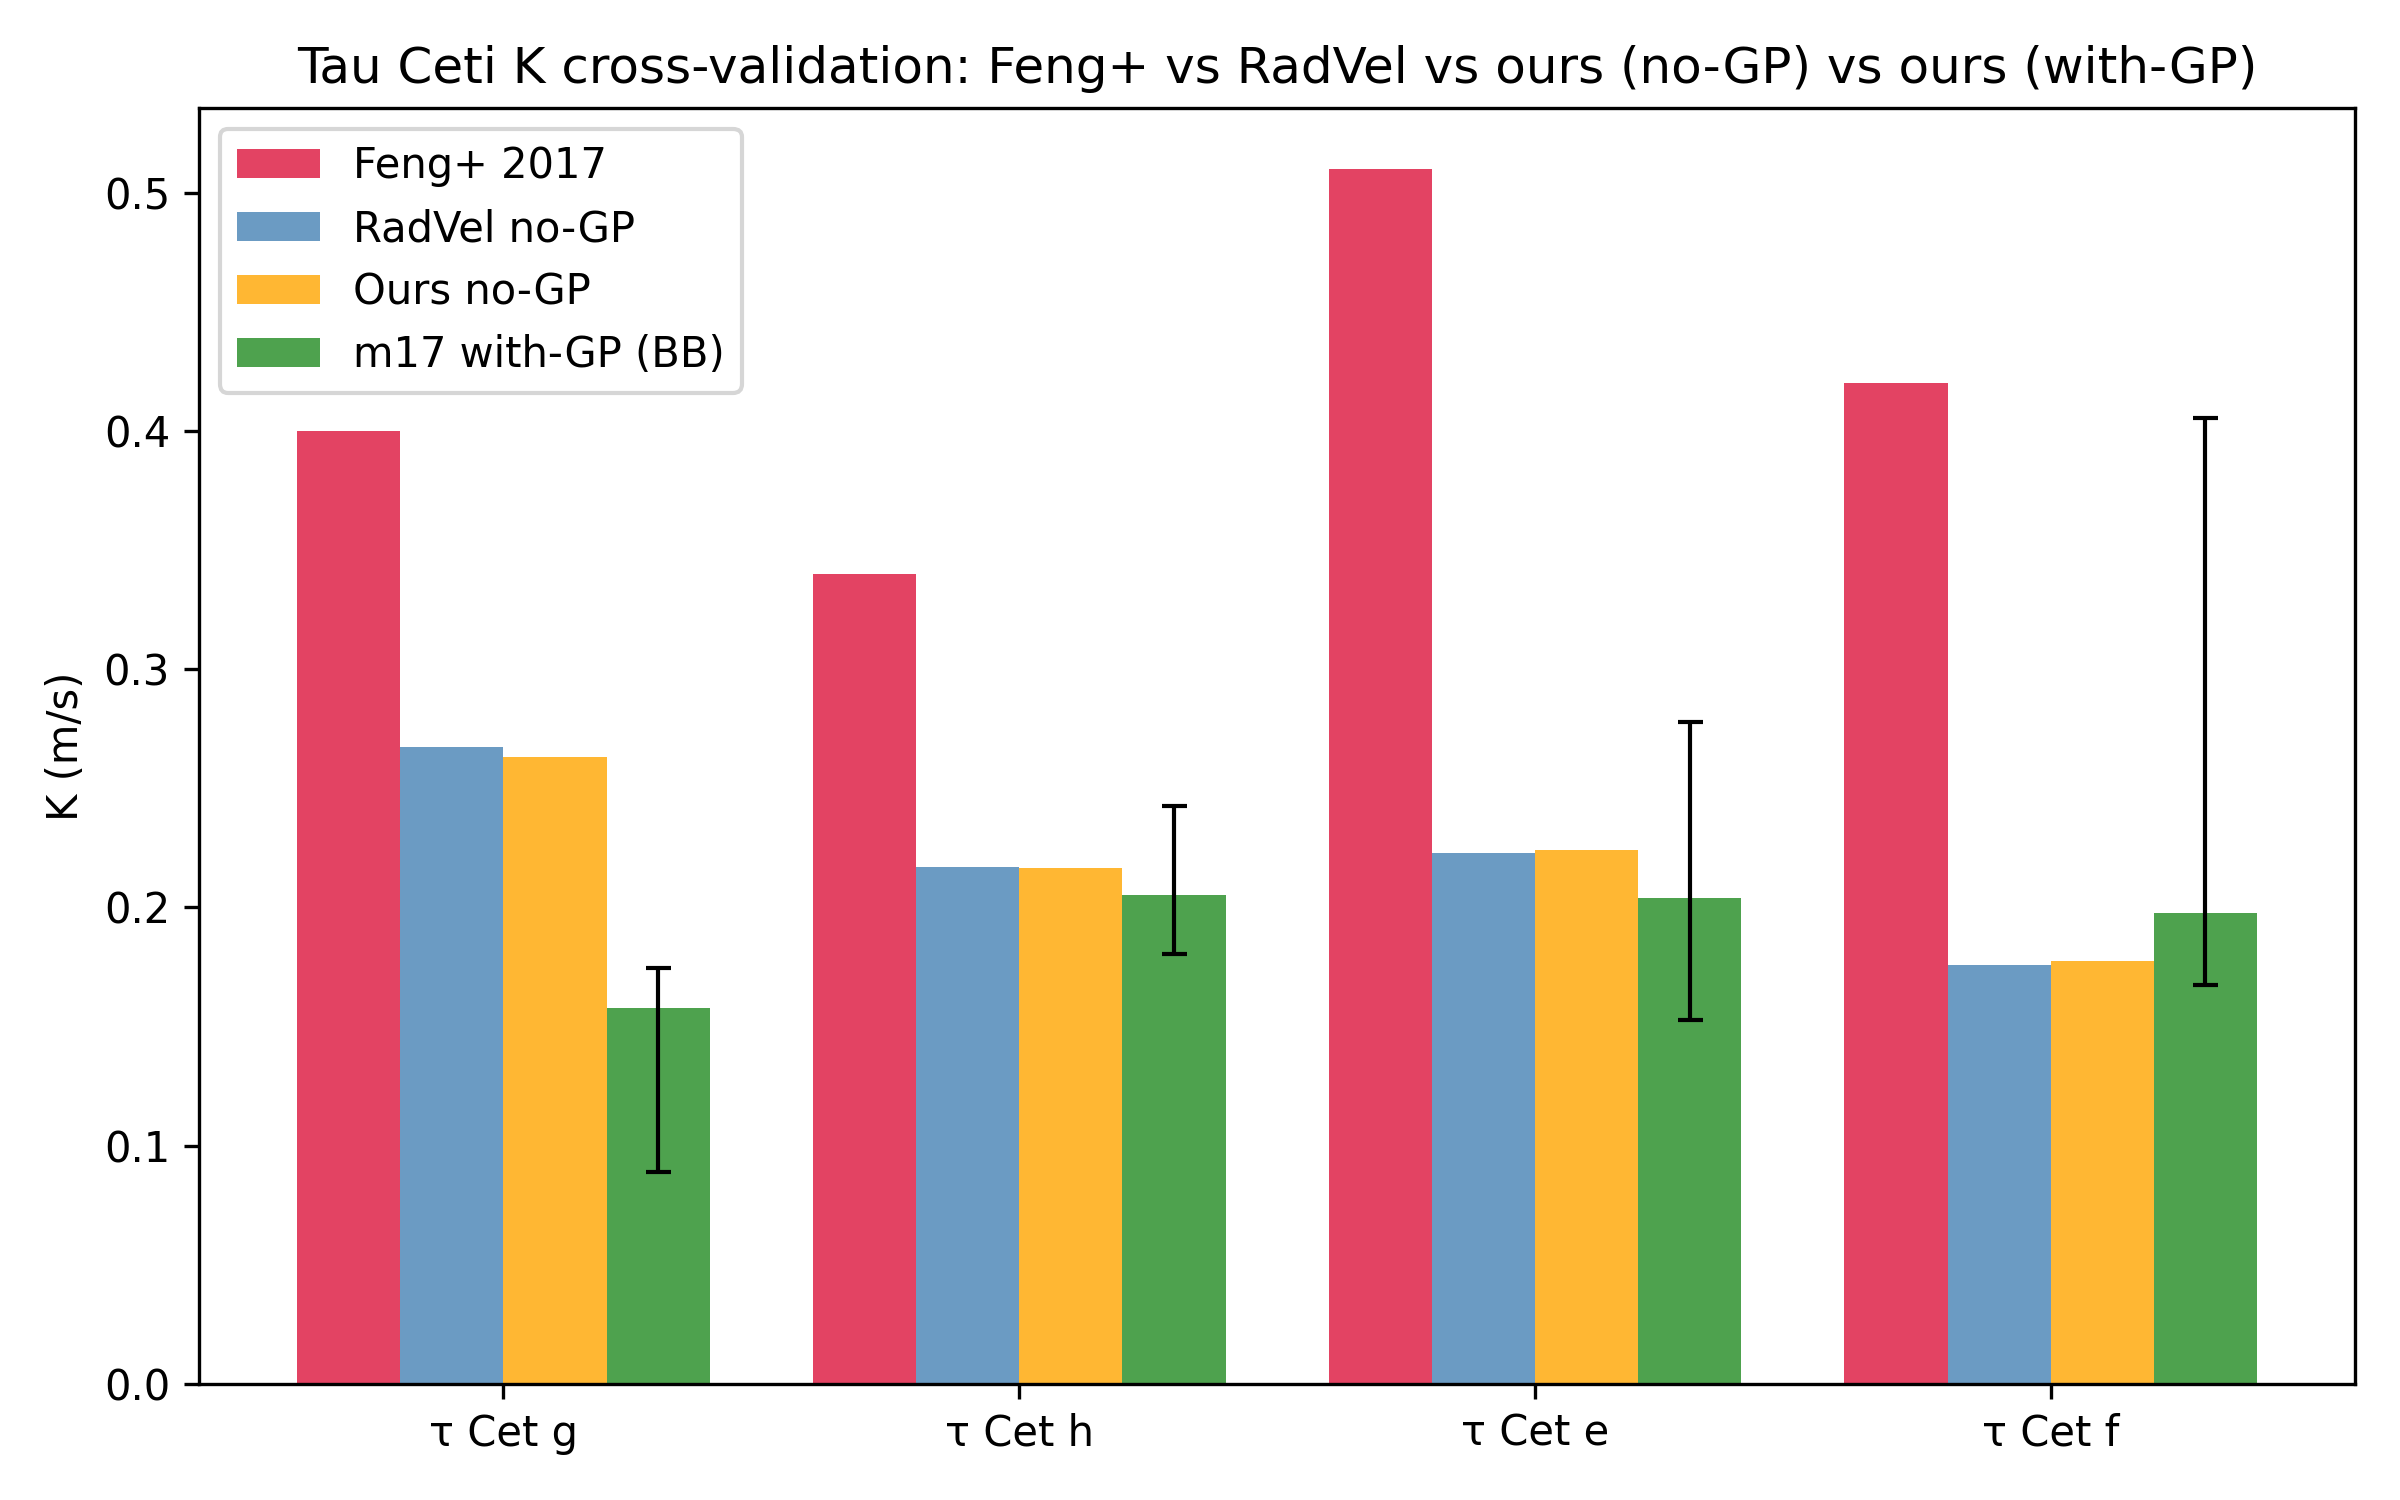
\includegraphics[width=0.75\textwidth]{k_comparison.png}
\caption{Recovered RV semi-amplitudes for the four $\tau$~Cet candidates. Crimson: \citet{Feng2017}. Blue / orange: identical \texttt{RadVel} and our-pipeline no-GP fits at fixed Feng+ periods and $e\!=\!0$ (agreement to 1.5\%). Green: our converged $n_{\rm live}\!=\!2000$ dynesty fit with the activity GP enabled; error bars are 16th--84th percentile. The K-deficit relative to \citet{Feng2017} is robust to pipeline choice and only weakly dependent on activity-GP modelling.\label{fig:k}}
\end{figure}

\begin{deluxetable}{lcccc}
\tabletypesize{\footnotesize}
\tablecaption{Recovered RV semi-amplitudes $K$ (m\,s$^{-1}$).
\label{tab:k}}
\tablehead{\colhead{Cand.} & \colhead{\citet{Feng2017}} & \colhead{\texttt{RadVel} no-GP} & \colhead{Ours no-GP} & \colhead{Ours, with GP}}
\startdata
g & 0.40 & 0.267 & 0.263 & $0.16^{+0.02}_{-0.07}$\\
h & 0.34 & 0.217 & 0.217 & $0.21^{+0.03}_{-0.02}$\\
e & 0.51 & 0.223 & 0.224 & $0.20^{+0.07}_{-0.05}$\\
f & 0.42 & 0.176 & 0.177 & bimodal: 0.20 / 0.40\\
\enddata
\tablecomments{\texttt{RadVel} and "Ours no-GP" use fixed Feng+ periods and $e\!=\!0$. "Ours, with GP" uses the converged nested-sampling fit at $n_{\rm live}\!=\!2000$ with free $P$ and $e$.}
\end{deluxetable}

\textbf{Bayes-factor reversal.} An initial five-rung evidence ladder at $n_{\rm live}\!=\!500$ preferred $k\!=\!3$ (g+h+e) over $k\!=\!4$ (g+h+e+f) by Bayes factor 3.1, with a $k\!=\!3$ posterior model probability of 60\% under a uniform prior on $k$. Re-running the headline $k\!=\!3$ and $k\!=\!4$ rungs at $n_{\rm live}\!=\!2000$ reversed the verdict: $\Delta \log Z_{3-4} = -0.67$, BF $\sim$ 2 in favour of $k\!=\!4$. Per-parameter posterior widths inflated by factors of 25--100$\times$ between the two convergence levels, and the absolute $\log Z$ values shifted by 9.5--11.3~nats per rung asymmetrically. Both BF magnitudes are well below the Jeffreys "strong evidence" threshold of $\log{\rm BF} > 5$: \textbf{the data is essentially indifferent between three and four planets at convergence}, consistent with the bimodal $K_f$ posterior.

We diagnose this as the \texttt{DynamicNestedSampler}'s posterior-focused refinement over-concentrating on the deepest mode at insufficient $n_{\rm live}$ in moderate-dimensional (39-D) problems. Practitioners working on similar low-amplitude RV systems should be cautious: parameter uncertainties reported from $n_{\rm live} \lesssim 1000$ \texttt{dynesty} runs may be substantially underestimated.

\section{Discussion}

The systematic K-deficit relative to \citet{Feng2017} is robust to pipeline choice (\texttt{RadVel} agreement to 1.5\%) and only weakly dependent on activity-GP modelling. It therefore lives either in methodology (Feng+'s priors, moving-average noise model, instrument subset, or per-epoch versus nightly binning) or in data access (proprietary records not available in DACE public mode). An apples-to-apples reproduction of the Feng+ pipeline on the current dataset would adjudicate.

For the planetary system itself, the conservative reading is: $\tau$~Cet~g (P~$\approx$~21~d), h (43~d), and e (161~d) are confirmed at $K \approx 0.16$--$0.21$~m\,s$^{-1}$; candidate~f is statistically indeterminate from the RV data alone, with the activity GP and the planet term competing to absorb the same $\sim$700-d signal. Resolving f will require independent observations.

\section*{Acknowledgements}

This research has made use of the DACE platform developed in the frame of PlanetS (\url{https://dace.unige.ch}). Analysis benefited substantially from work performed by the Anthropic Claude language model (Opus 4.7) acting as a research assistant: code authoring, milestone-by-milestone analysis, and detection of methodological errors. The complete development log (23 milestone reports, $\sim$5\,500 lines of analysis code, source repository) is publicly available at \url{https://github.com/phwizard/beholder-tau-ceti}, archived on Zenodo \dataset[doi:10.5281/zenodo.20613120]{https://doi.org/10.5281/zenodo.20613120}.

\software{dynesty \citep{Speagle2020}, RadVel \citep{Fulton2018}, celerite2 \citep{Foreman-Mackey2017}, numpy, scipy, astropy}

\bibliographystyle{aasjournal}

\begin{thebibliography}{}

\bibitem[Baliunas et al.(1996)]{Baliunas1996} Baliunas, S.~L., et al.\ 1996, \apj, 457, L99

\bibitem[Buchschacher et al.(2015)]{Buchschacher2015} Buchschacher, N., et al.\ 2015, ADASS XXIV, 495, 7

\bibitem[Feng et al.(2017)]{Feng2017} Feng, F., et al.\ 2017, \aj, 154, 135

\bibitem[Foreman-Mackey et al.(2017)]{Foreman-Mackey2017} Foreman-Mackey, D., et al.\ 2017, \aj, 154, 220

\bibitem[Fulton et al.(2018)]{Fulton2018} Fulton, B.~J., Petigura, E.~A., Blunt, S., \& Sinukoff, E.\ 2018, \pasp, 130, 044504

\bibitem[Speagle(2020)]{Speagle2020} Speagle, J.~S.\ 2020, \mnras, 493, 3132

\end{thebibliography}

\end{document}
